\section{Stability Analysis}

\subsection{Introduction}
\par In this section we will lay out a framework for analysing the stability of a numerical method.\\
To begin, we will introduce the concept of the stability function.\\
We will show how it can be used to define a stability region.\\
We will explore the stability region as the set of values for which a numerical method is stable.\\
Finally, we will extend this framework to view the stability of a numerical method in the context of complex time steps.\\

\subsection{Numerical Method: Forward Euler}

\par Let's consider a simple numerical method applied to the Exponential Decay Problem.\\
The Forward Euler method is a first-order numerical method for solving ODEs with a given initial condition.\\
Its algorithm can be defined as:
\[ y(t_{j+1}) = y(t_j) + h y'(t_j)\]
Where $h$ is the time step and $y_j$ is the numerical solution at time $t_j$, $j$ steps on from $t_0=0$.\\
This means $t_j = hj$.\\

\par For the Exponential Decay Problem, the Forward Euler method can be written as:
\[ y_{j+1} = y_j + h \lambda y_j \quad \text{where} \quad y_0 = 1\]
This gives us the following algorithm:
\[ y_{j+1} = (1 + h \lambda) y_j\]
This gives an approximation of the exact solution at time $t_j$ as follows:
\[ y_{j} = {(1 + h \lambda)}^j y_0 = {(1 + h \lambda)}^j = y(t_j) = y(hj) \approx e^{\lh j}\]

\par We can see that the Forward Euler method is stable if $|1 + h \lambda| < 1$;\\
both the exact solution and our approximation will decay to zero as $t \rightarrow \infty$.\\
The stability is dependent on the time step $h$ and the value of $\lambda$.\\
We can write this as $s(\lambda, h) = 1 + h \lambda$.\\
By analysing $s$ for different values of $\lambda$ and $h$,\\
we can infer the stability of the Forward Euler method for the Exponential Decay Problem.\\
We call $s$ the \term{stability function} of the Forward Euler method.

\subsection{The Stability Function and corresponding Stability Region}
\par By the same methodology, we can define the stability function for any numerical method by writing the algorithm in the form $y_{j+1} = s(\lambda, h) y_{j}$.\\
$s(\lambda, h)$ is the \term{stability function} of the numerical method with a time step $h$.\\
\textbf{Note:} This is equivalent to $y_{j} = {s(\lambda,h)}^{j} y_0$

\par The \term{stability region} of a numerical method is the set $S = \Big\{ (\lambda, h) \;\Big|\; |s(\lambda, h)| < 1\Big\} \subset \bC$\\
This follows from the definition of stability for our Exponential Decay Problem;\\
a method is stable if the numerical solution decays to zero as $t \rightarrow \infty$.\\
Clearly, $\Lim{j \rightarrow \infty}y_{j} = \Lim{j \rightarrow \infty}{s(\lambda,h)}^{j} y_0 = 0 \iff |s(\lambda, h)| < 1$.
Now, let's explore some examples of stability regions for different numerical methods.

\newpage
\subsubsection{Stability Region for Euler's Forward Method}
\begin{multicols}{2}
Euler's Forward Method has the stability function
\[s(\lambda, h) = 1 + \lh = \sum\limits_{n=0}^{1} \frac{{(\lh)}^n}{n!} = M(y) + \mathcal{O}((\lh)^2)\]
The corresponding stability region is 
\[S = \Big\{ (\lambda, h) \;\Big|\; |1 + \lh| < 1\Big\}\]
We can see this region plotted in red on the right; an open unit circle centred at $-1$.\\

For a given $\lambda \in \bC$, the method is stable for any step-size $h \in \bR$ such that $|1 + \lh| < 1$.\\

\par Expanding $\lambda = a + bi$, we get the restriction
\[|1 + (a + bi)h| < 1 \quad \implies \quad |(1+ah) + (bh)i| < 1\] 
\[\implies \quad a^2h^2 + 2ah + b^2h^2 < 0\]
\[a, b, h \in \bR \implies (a^2 +b^2)h^2 > 0\] 
\[\implies 2ah < 0 \text{ and } ||2ah|| > (a^2 + b^2)h^2\]
This aligns with our intuition for the problem;
\begin{itemize}
	\item[$\cdot$] For the exponential to decay,\\
	      we must have $Re(\lambda) = a < 0$.
	\item[$\cdot$] $h$ must be positive, as it is a time step.
\end{itemize}
\columnbreak{}
\vspace*{\fill}
\begin{center}
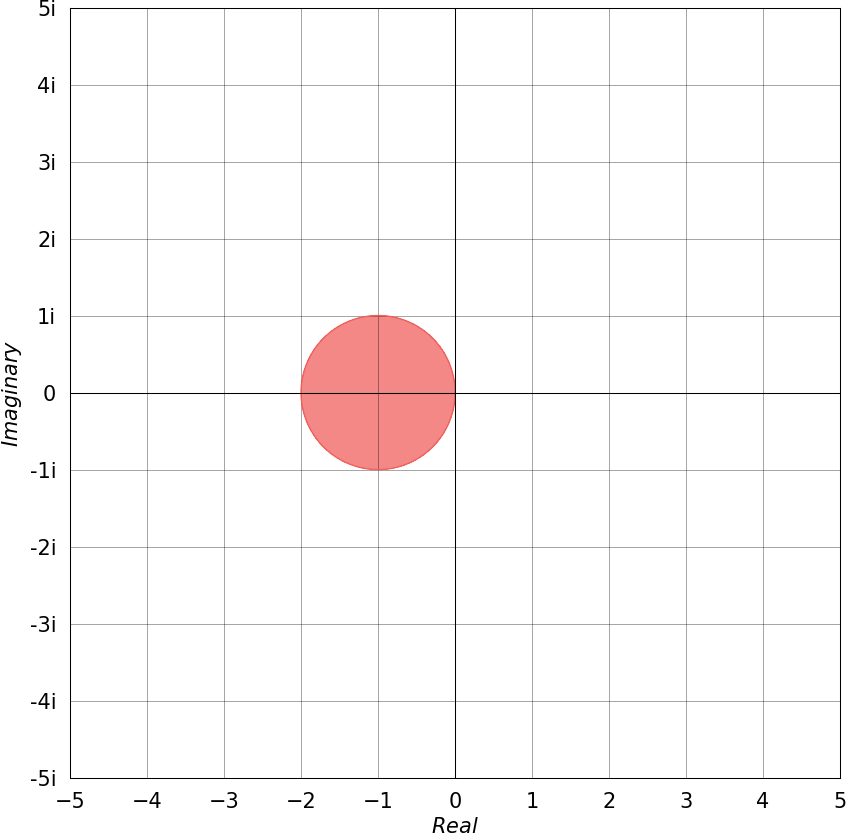
\includegraphics[width=0.49\textwidth]{Stability Regions/Graphs/Real 1-Step/Euler's Forward.png}
\end{center}
\vspace*{\fill}
\end{multicols}
Moreover, 
\[0 < (a^2 +b^2)h^2< ||2ah|| \quad\implies\quad 0 < h < \frac{||2a||}{a^2 + b^2} \quad\implies\quad 0 < h < \frac{2 ||Re(\lambda)||}{{|\lambda|}^2}\]
This is also intuitive; if we imagine $\lambda$ growing linearly, $h$ must shrink quadratically so that their product $\lh$ stays inside the stability region.\\
%\textbf{Note to self: This feels similar to the inversion of a point through a circle in $\bC$.}

\subsubsection{Stability Region for Euler's Backward Method}
\begin{multicols}{2}
\vspace*{\fill}
\begin{center}
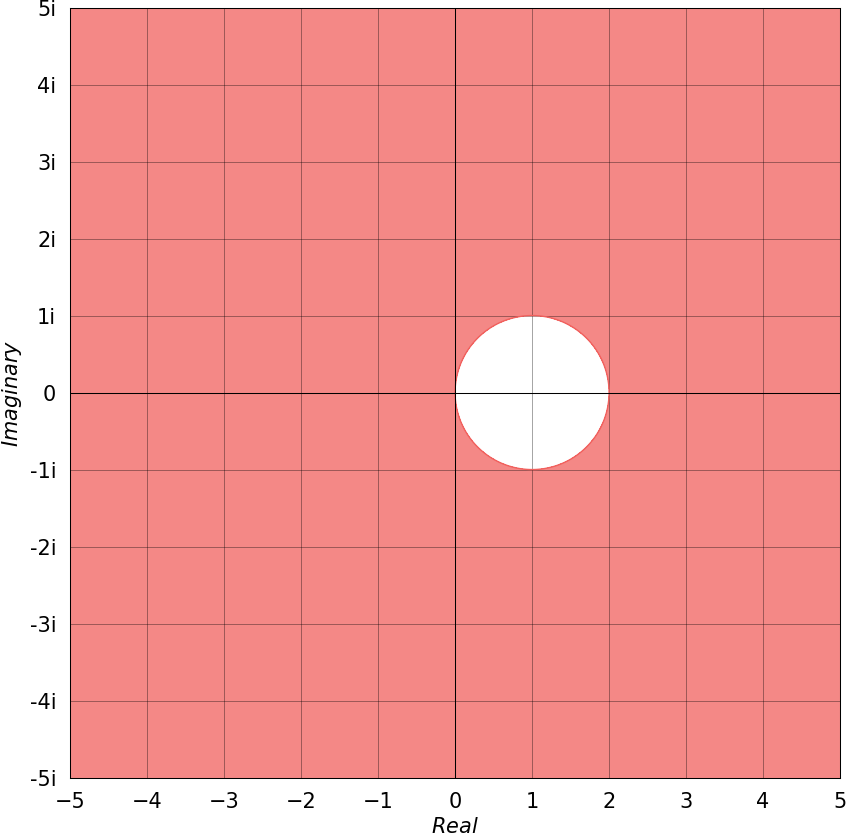
\includegraphics[width=0.49\textwidth]{Stability Regions/Graphs/Real 1-Step/Euler's Backward.png}
\end{center}
\vspace*{\fill}
\columnbreak{}
Euler's Backward Method can be written as
\[y_{j+1} = y_j + h.y'(t_{j+1})\]
\[\implies y_{j+1} = y_j + h(\lambda y_{j+1}) \implies y_{j+1} = \frac{1}{1 - \lh}y_j\]
Thus, the stability function is
\[s(\lambda, h) = \frac{1}{1 - \lh}\]
The corresponding stability region is
\[S = \Big\{ (\lambda, h) \;\Big|\; \left|\frac{1}{1 - \lh}\right| < 1\Big\}\]
This is plotted in red on the left; the region outside a unit circle centred at $1$.\\
The white region of instability is exactly the stability region for Euler's Forward Method, flipped about Imaginary axis.\\

\par We could run through the same algebraic proceedure as before, expanding $\lambda$ and rearranging, and we would find that 
\[h > \frac{2 Re(\lambda)}{{|\lambda|}^2}\]
\end{multicols}
This is a more lax restriction than the $0<h$ that we have already established.\\
In fact, this tells us that any positive $h$ will give a stable solution, regardless of the value of $\lambda$.\\
This is a property called \term{Absolute Stability} or \term{A-Stability}.\\
This is often characterised by a stability region that covers the entire left half-plane, as we see here.\\

\subsubsection{Stability Region for Runge-Kutta 4}
\begin{multicols}{2}
\vspace*{\fill}

Runge-Kutta 4 can be written as
\[y_{j+1} = y_j + \frac{h}{6}(k_1 + 2k_2 + 2k_3 + k_4)\]
Where $\phi(t,y) = y'(t) = \lambda y$
\begin{flalign*}
	k_1 &= \phi(t_j, y_j) \quad &k_2 = \phi(t_j + \frac{h}{2}, y_j + \frac{h}{2}k_1) && \\
	k_3 &= \phi(t_j + \frac{h}{2}, y_j + \frac{h}{2}k_2) \quad &k_4 = \phi(t_j + h, y_j + hk_3) &&
\end{flalign*}
For the Exponential Decay Problem, we get
\[y_{j+1} = (1 + \lh + \frac{{(\lh)}^2}{2} + \frac{{(\lh)}^3}{6} + \frac{{(\lh)}^4}{24})y_j\]
The stability function is
\[s(\lambda, h) = \sum\limits_{n=0}^{4}\frac{{(\lh)}^n}{n!} = M(y) + \mathcal{O}((\lh)^5)\]
The corresponding stability region is
\[S = \Big\{ (\lambda, h) \;\Big|\; \left|\sum\limits_{n=0}^{4}\frac{{(\lh)}^n}{n!}\right| < 1\Big\}\]

\vspace*{\fill}
\columnbreak{}
\begin{center}
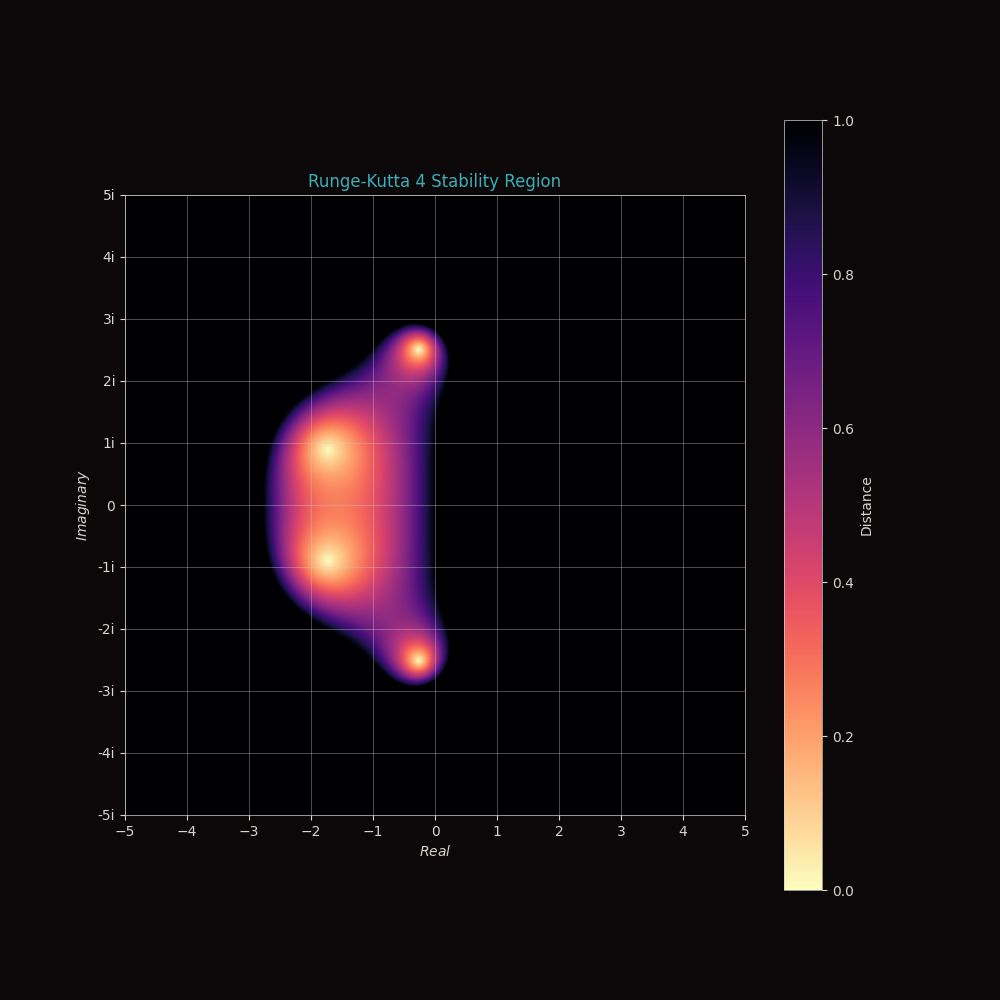
\includegraphics[width=0.49\textwidth]{Stability Regions/Graphs/Real 1-Step/Runge-Kutta 4.png}
\end{center}
\end{multicols}

\newpage
\subsection{Interpretation of Stability Regions}

\par The stability region $S = \Big\{ (\lambda, h) \;\Big|\; |s(\lambda, h)| < 1\Big\} \in \bC$ is a set of values for which a numerical method is stable for the Exponential Decay Problem.\\
We always restrict $h \in {\bR}^{+}$, as it is a time step.\\
We have two separate cases for $\lambda$:
\begin{itemize}
	\item[$\cdot$] $\lambda \in {\bR}^{-}$:\;\; $S$ corresponds to $\big\{{s(\lambda, h)}^2 < 1\big\}$. \;\; Of course, $\lambda, h \in \bR \implies S \subset \bR$.
	\item[$\cdot$] $\lambda \in \bC\setminus\bR$ with $Re(\lambda) < 1$:\;\; $S$ corresponds to $\Big\{\big(s(\lambda, h)\big)\big(\,\overline{s(\lambda, h)}\,\big) < 1\Big\}$.
\end{itemize}

\par From here, one can derive bounds on $h$ for a given value of $\lambda$, or vice versa.\\
We did this with Euler's Forward and Backward methods above.\\
The Runge-Kutta 4 method is more complex, as the two cases of $\lambda$ each give a polynomial of degree 8.\\

\par Below we have graphs for the cases where $\lambda$ is real or complex,\\
the same as we introduced for the Exponential Decay Problem.\\
In black is the exact solution. In colour are the numerical solutions due to the method in question.\\
These $(\lambda, h)$ pairs were found by first picking a value of $\lambda$ and then finding $h$ values which met the stability condition.\\
In green $(\lambda, h) \in S$.\\
In red $(\lambda, h) \notin S$.

\subsubsection{Euler's Forward Method}
\begin{multicols}{2}
	\begin{center}
	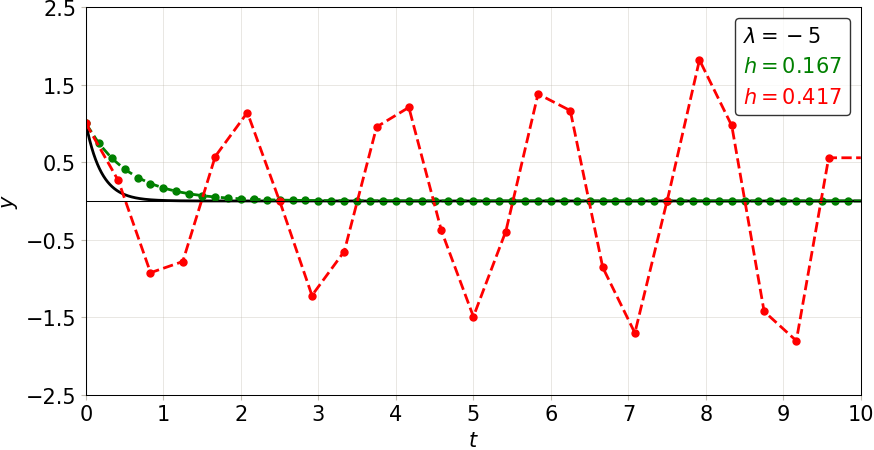
\includegraphics[width=0.49\textwidth]{Exponential Decay/Exact vs Method/Euler's Forward real-real.png}
	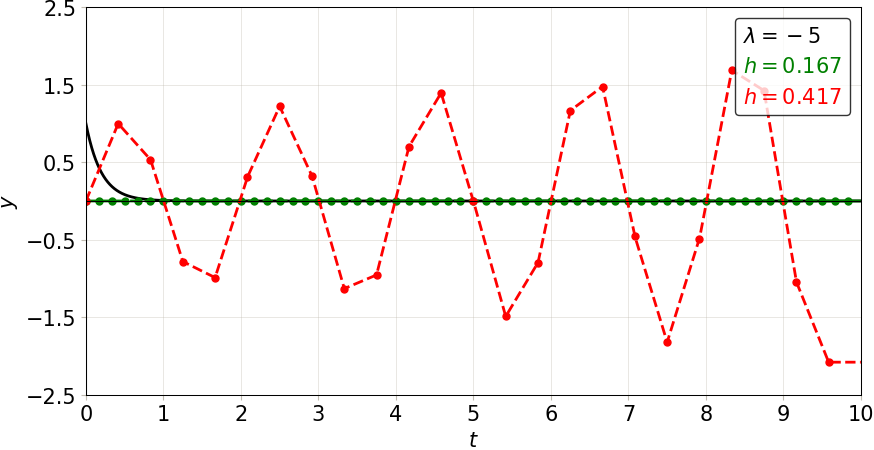
\includegraphics[width=0.49\textwidth]{Exponential Decay/Exact vs Method/Euler's Forward real-imag.png}
	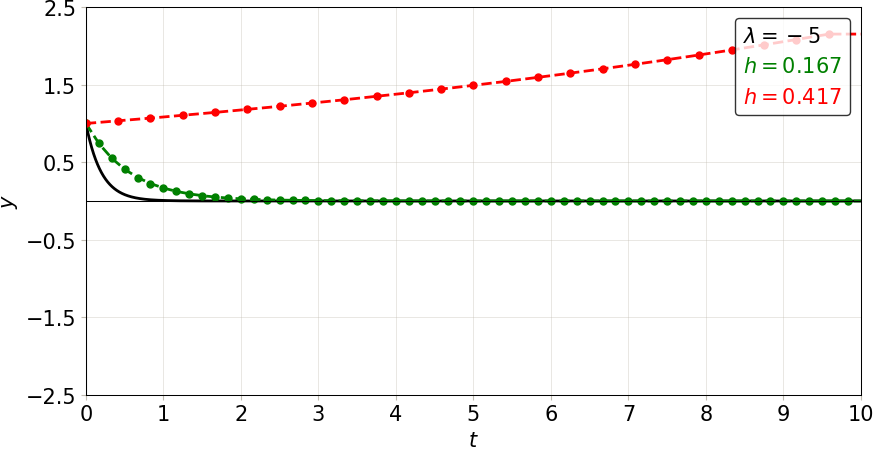
\includegraphics[width=0.49\textwidth]{Exponential Decay/Exact vs Method/Euler's Forward real-mag.png}
	\end{center}
\columnbreak{}
	\par On the left are the aforementioned graphs for\\
	Euler's Forward Method with $\lambda \in \bR^{-}$.\\
	We have 3, as for the unstable $h=\frac{5}{12}$ the method gives complex outputs.\\
	From the top down, the graphs show the real part, the imaginary part and the magnitude of the numerical solution.\\
	In all 3, the black is real, and only, part of the exact solution.\\
	We can notice for the imaginary part that the green, stable $h = \frac{1}{6}$ is $0$; this is strictly real.\\
	\begin{center}
        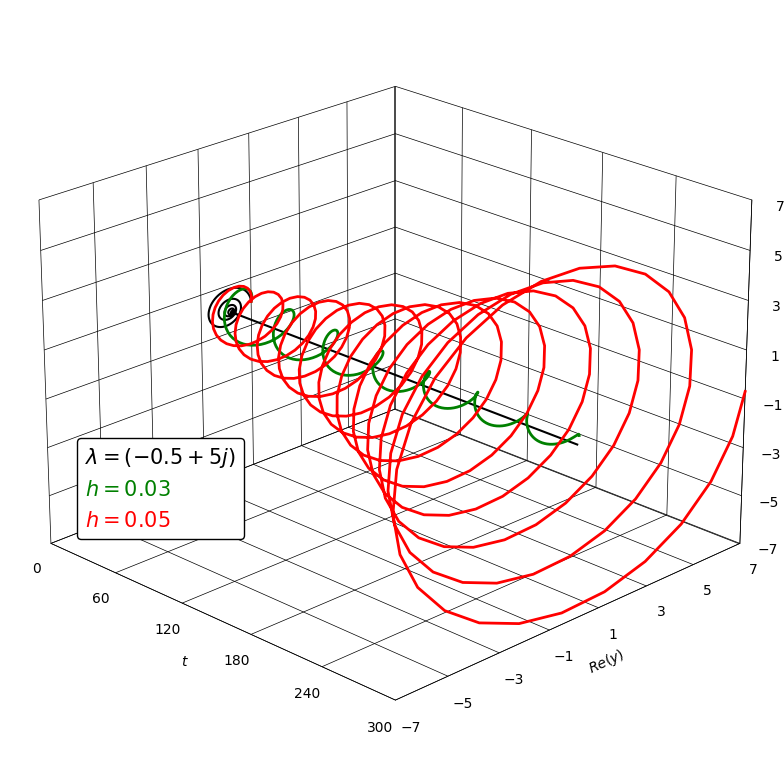
\includegraphics[width=0.49\textwidth]{Exponential Decay/Exact vs Method/Euler's Forward complex.png}
        \end{center}
\end{multicols}
\par On the right is the case where $\lambda \in \bC$. The exact solution decays quickly in black, very close to the $t=0$ plane.\\
The green, valid $h$ value converges as $t$ increases, but the red, invalid $h$ value diverges.\\
While this 3D graph might not be the clearest, it took quite a lot of messing with values of $h$ and $\lambda$ to find one so demonstrative.\\
The reader is encouraged to play with `/Python/Exponential Decay/Exact vs Method.py' in the GitHub repository~\cite{GitHub_Repo} to see for themselves.\\
This has the added benefit of allowing you to rotate the graph to see the behaviour from different angles.

\subsubsection{Euler's Backward Method}
As mentioned before, Euler's Backward Method is A-Stable.\\
This means that for any $\lambda \in \bC$, the method is stable for any $h \in \bR^{+}$.\\
As a result, there is no choice of $(\lambda, h)$ that will give us a divergent graph.\\
What happens if we relax our restrictions on $h$ and $\lambda$ to attain a value in our white circle of instability, you ask?\\
If the $\lh$ value is in the white circle, we are looking at a growing exponential.
Is cuma liom.
Instead, these graphs show two different valid $h$ values for the same $\lambda$ value.\\
These use the same values as we had for Euler's forward Method.\\
\begin{multicols}{2}
\begin{center}
	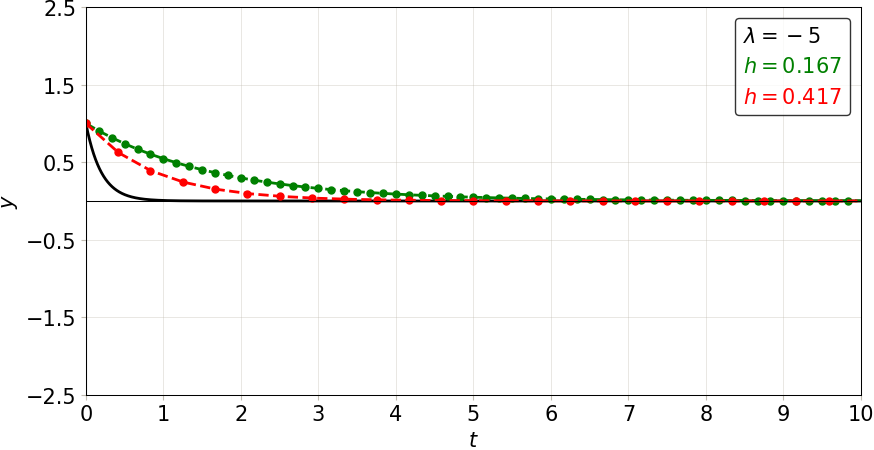
\includegraphics[width=0.49\textwidth]{Exponential Decay/Exact vs Method/Euler's Backward real-real.png}
	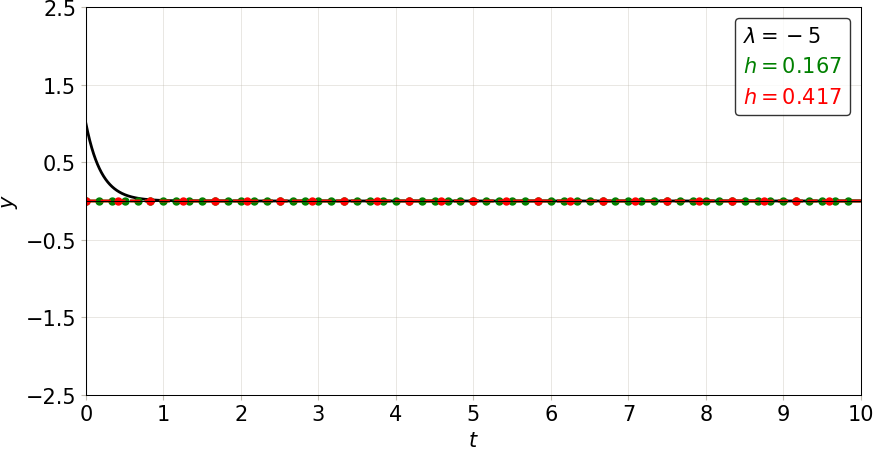
\includegraphics[width=0.49\textwidth]{Exponential Decay/Exact vs Method/Euler's Backward real-imag.png}
	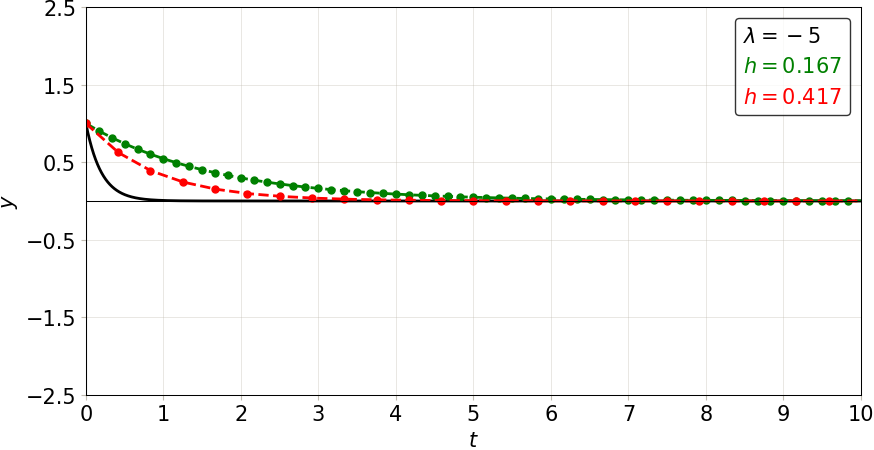
\includegraphics[width=0.49\textwidth]{Exponential Decay/Exact vs Method/Euler's Backward real-mag.png}
\end{center}
\columnbreak{}
\begin{center}
	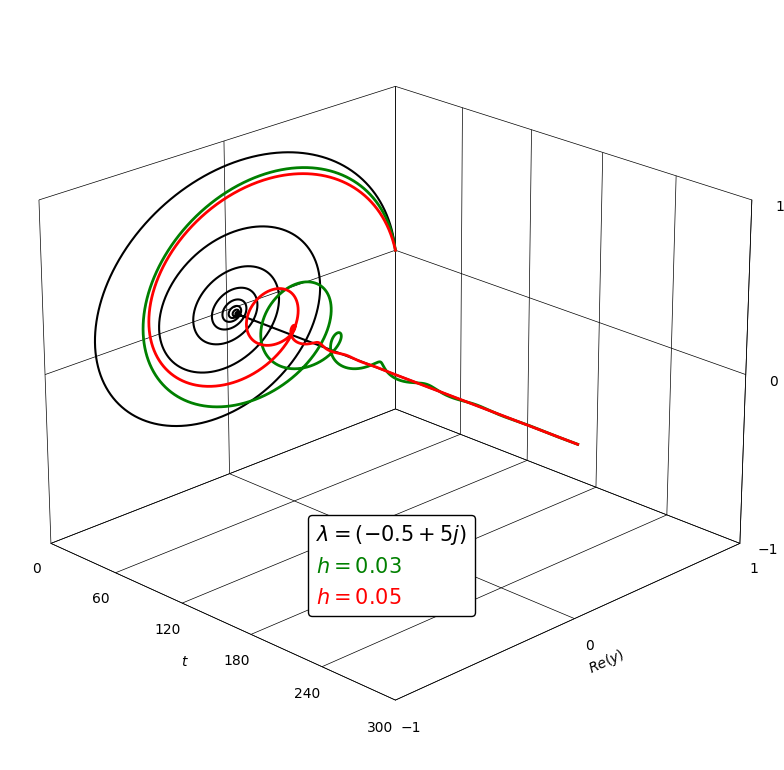
\includegraphics[width=0.49\textwidth]{Exponential Decay/Exact vs Method/Euler's Backward complex.png}
\end{center}
	In the $\lambda \in \bR$ case, the numerical solution converges to the exact solution for both step sizes.\\
	On the second, imaginary, graph, we can see that both numerical methods are constantly $0$ as they are strictly real.\\
	The magnitude graph is identical to the real graph, indicating the same behaviour.\\
	In the case where $\lambda \in \bC$, the method converges to the exact solution for both step sizes for both real and complex $\lambda$.\\
	There is no divergence, as we have already established.\\
	Interestingly, the method converges faster for the larger step size.\\
	\textbf{Should we explore this further? Like, this makes sense if you think about the stability eq, but it is also counter intuitive. I have graphs showing not only the stability regions, but the `density' for certain step sizes\ellipsis}
\end{multicols}
%\par Let $\lh = \alpha + \beta i$ for any $\alpha, \beta \in \bR$ and suppose $\left|\frac{1}{1 - \lh}\right| \geq 1$.\\
%This gives us
%\[\left|\frac{1}{1 - \lh}\right| = \left|\frac{1}{1 -(\alpha + \beta i)}\right| = \left|\frac{1}{(1 -\alpha) - \beta i}\right| = \left|\frac{1}{(1 -\alpha) - \beta i}\right| \cdot \left|\frac{(1 -\alpha) + \beta i}{(1 -\alpha) + \beta i}\right| = \left|\frac{(1 - \alpha) + \beta i}{{(1 - \alpha)}^2 + \beta^2}\right| \geq 1\]
%\[ \big({(1-\alpha)}^2 + \beta^2\big) \in \bR \quad\implies\quad \left|\frac{(1 - \alpha) + \beta i}{{(1 - \alpha)}^2 + \beta^2}\right| \;=\; \frac{\left|(1 - \alpha) + \beta i\right|}{{(1 - \alpha)}^2 + \beta^2} \;\geq\; 1 \quad\implies\quad \left|(1 - \alpha) + \beta i\right| \;\geq\; {(1 - \alpha)}^2 + \beta^2\]
%\[\implies \sqrt{{(1 - \alpha)}^2 + \beta^2} \;\geq\; {(1 - \alpha)}^2 + \beta^2 \quad \text{A contradiction!}\quad ( \text{Except if } \alpha = \beta = 0)\]
%Thus, even if we allow $\lambda, h \in \bC$, we cannot find values that will give us a divergent graph.\\
%There is no $(\lambda, h)$ that will land us within the white circle of instability!\\
\newpage
\subsubsection{Runge-Kutta 4}
\begin{multicols}{2}
\begin{center}
	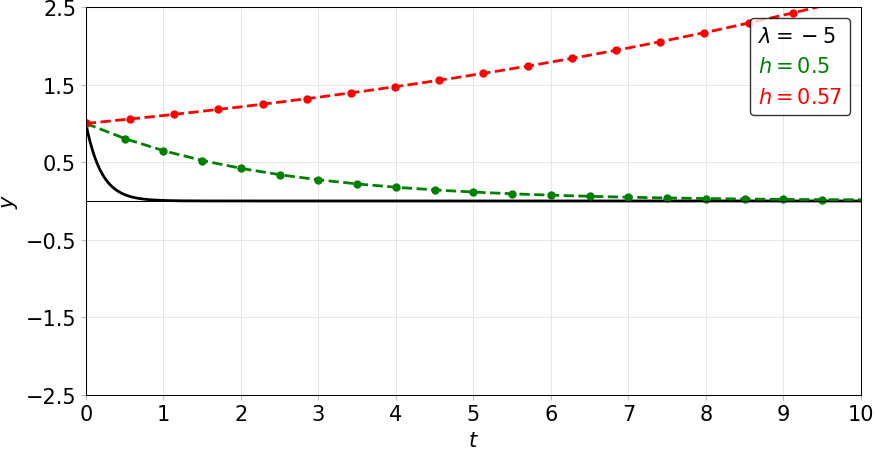
\includegraphics[width=0.49\textwidth]{Exponential Decay/Exact vs Method/Runge-Kutta 4 real-real.png}
	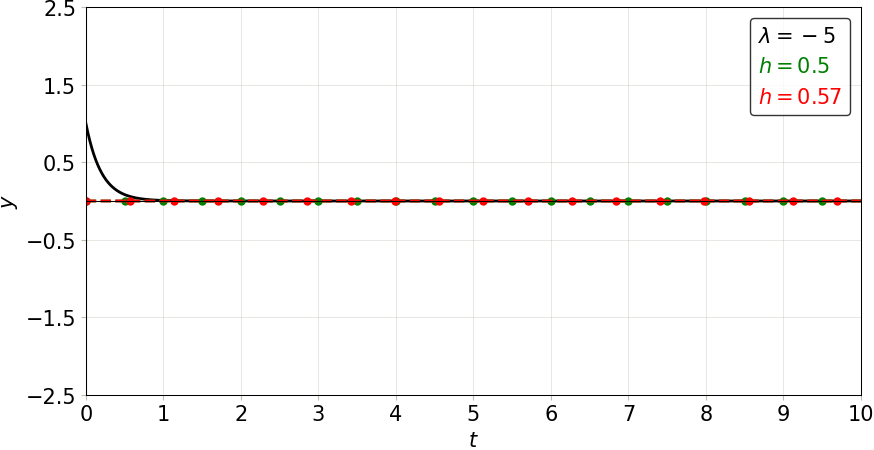
\includegraphics[width=0.49\textwidth]{Exponential Decay/Exact vs Method/Runge-Kutta 4 real-imag.png}
	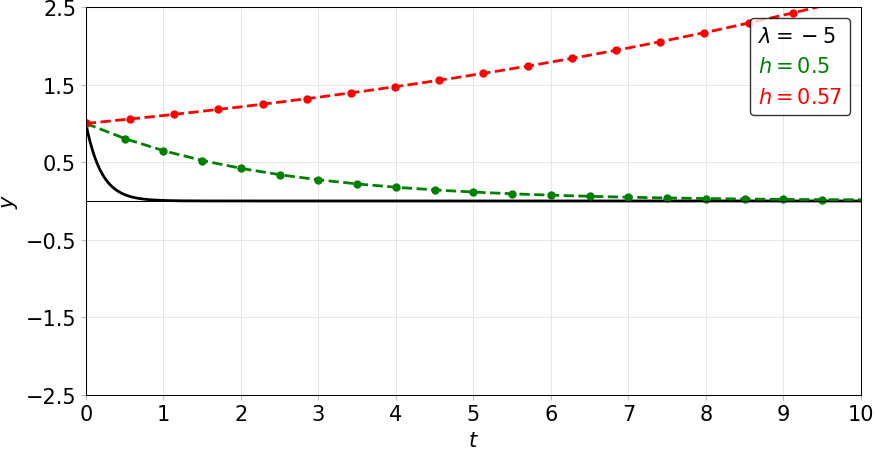
\includegraphics[width=0.49\textwidth]{Exponential Decay/Exact vs Method/Runge-Kutta 4 real-mag.png}
\end{center}
\columnbreak{}
\begin{center}
	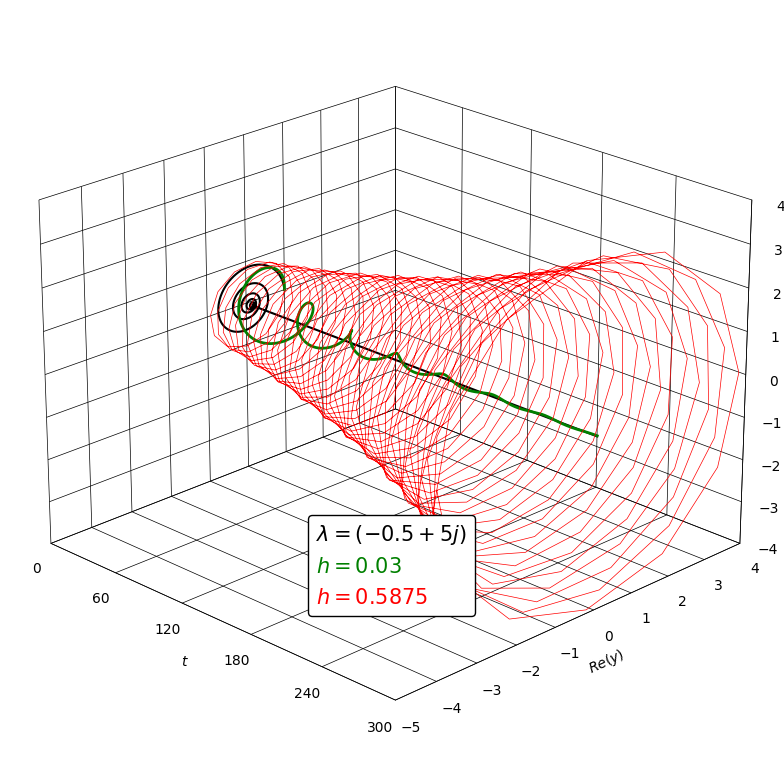
\includegraphics[width=0.49\textwidth]{Exponential Decay/Exact vs Method/Runge-Kutta 4 complex.png}
\end{center}
\end{multicols}
\subsection{Numerical Method: 2-step Abysmal Kramer-Butler Method}

\par This method was designed to be unstable for the sake of demonstration.\\
The algorithm is as follows:
\[y_{j+1} = y_{j-1} + h(4\phi(t_j,y_j)-2\phi(t_{j-1},y_{j-1}))\]
As we know the exact solution to our Exponential Decay problem is $y(t) = e^{\lambda t}$, we know $\phi(t,y) = \lambda y$.\\
This gives:\\
\[y_{j+1} = y_{j-1} + h(4\lambda y_j - 2\lambda y_{j-1})\]
Simplified:\\
\[y_{j+1} = 4\lh y_j + (1-2\lh) y_{j-1}\]
%FURTHER DERIVATION ON WHITEBOARD - Aim: Get method in terms of $y_{j}$, $y_1$ and $y_0$ only.\\
